\documentclass[a4paper,12pt]{article}

\usepackage{cmap}          % поиск в PDF
\usepackage{mathtext}         % русские буквы в формулах
\usepackage[T2A]{fontenc}      % кодировка
\usepackage[utf8]{inputenc}      % кодировка исходного текста
\usepackage[english,russian]{babel}  % локализация и переносы
\usepackage[left=2cm,right=2cm,top=2cm,bottom=2cm]{geometry}
\usepackage{amsfonts,amssymb,amsthm,mathtools} % AMS
\usepackage{amsmath}
\usepackage{icomma} % "Умная" запятая: $0,2$ --- число, $0, 2$
\usepackage{graphicx}
\usepackage{wrapfig} % картинка в тектсе
\usepackage{caption} % убирается номер у подписей caption*{}
\usepackage{csquotes} % цитаты
\usepackage{multirow} % для жестких таблиц
\usepackage{hhline}
\usepackage{indentfirst} % абзацный отступ после section
\usepackage{epigraph} % эпиграф
\usepackage{tikz}
\usepackage{pgfplots}
\usepackage[export]{adjustbox}
\usepackage{tabularx}
\usepackage{float}
\usepackage{longtable}


\graphicspath{{pictures/}}
\begin{document}
	\pagenumbering{gobble}
	\pagenumbering{arabic}
	

	\title{\textbf{Исследование взаимной диффузии газов. (2.2.1)}}
	\author{Зайнуллин Амир Б05-206}

	\maketitle

	\section{Аннотация}
	
	\textbf{Цель работы:} 1) регистрация зависимости концентрации гелия в воздухе от времени с помощью датчиков теплопроводности при разных начальных давлениях смеси газов; 
    2) определение коэффициента диффузии по результатам измерений. \\
	\textbf{В работе используются:} термостат, герметический сосуд, заполненный водой, отсчётный микроскоп.
	
	
	\section{Теоретические сведения}
	
	Диффузией называют самопроизвольное взаимное проникновение веществ друг в друга, происходящее вследствие хаотичного теплового движения молекул.
	
	Диффузия в системе, состоящей из двух компонентов $ a $ и $ b $ (бинарная смесь), подчиняется закону Фика: плотности потока компонентов $ j_{a,b} $ (количество частиц, пересекающих единичную площадку в единицу времени) пропорциональны градиентам их концентраций $ \nabla n_{a,b}$
	
	\[ j_a = -D\dfrac{\partial n_a}{\partial x}, \quad j_b = -D\dfrac{\partial n_b}{\partial x}, \]
	где $ D $ -- коэффициент взаимной диффузии компонентов.
	
	В случае работы с данной установкой можно считать, что диффузионный поток одинаков в любом сечении трубки, соединяющей сосуды $V_1$ и $V_2$. Следовательно:
	
	В данной работе исследуется взаимная диффузия гелия и воздуха. Поэтому для любых изменений концентраций справедливо $ \Delta n_{He}=-\Delta n_{\text{в}} $. Следовательно, достаточно ограничиться описанием диффузии одного из компонентов, например гелия $ n_{He} $:
	
	\begin{equation}
		j_{He}=-D\dfrac{\partial 	n_{He}}{\partial x}.
	\end{equation}
	
	Приведём теоретическую оценку для коэффициента диффузии. В работе концентрация гелия, как правило, мала $ (n_{He} \ll n_\text{в}) $. Кроме того, атомы гелия существенно легче молекул, составляющих воздух ($ \mu_{He} \ll \mu_{O_2}, \mu_{N_2} $), значит и их средняя тепловая скорость велика по сравнению с остальными частицами. Поэтому перемешивание газов в работе можно приближенно описывать как диффузию примеси лёгких частиц $ He $ на практически стационарном фоне воздуха. Коэффициент диффузии в таком приближении равен
	
	\begin{equation}
		D=\dfrac{1}{3}\lambda 	\overline{v},
	\end{equation}
	
	где $ \overline{v}=\sqrt{\frac{8RT}{\pi \mu}} $ -- средняя тепловая скорость частиц примеси, $ \lambda = \frac{1}{n_0\sigma} $ -- их длина свободного пробега, $ n_0 $ -- концентрация рассеивающих центров (фона), $ \sigma $ -- сечение столкновения частиц примеси с частицами фона.
	
    Формула продолжает работать если $ \lambda = \dfrac{1}{(n_{He} + n_в)\sigma} = \dfrac{k_{б} T}{P \sigma}$

	Таким образом, теория предсказывает, что коэффициент диффузии бинарной смеси обратно пропорционален давлению в системе $ D \propto 1/P $, и не зависит от пропорций компонентов, что и предлагается проверить в работе экспериментально.
	
    Применяя закон Фика в трубке, получим

    \[ j=-D\frac{\partial n}{\partial x} = const \]

    \begin{equation}
    n(x) = \frac{\Delta n}{L} x
    \end{equation}
    и плотность потока частиц всюду постоянна и равна

    \begin{equation}
    j=-D\frac{\Delta n}{L},
    \end{equation}
    где $ \Delta n = n_2-n_1 $ -- разность концентраций гелия на концах трубки.

    Полное число частиц примеси в сосудах равно соответственно $ N_1=n_1V $ и $ N_2=n_2V $. Произведение плотности потока на площадь сечения трубки $ S $ даёт количество частиц, пересекающих в единицу времени любое поперечное сечение трубки. Поэтому

    \begin{equation}
    \frac{dN_1}{dt}=jS, \quad \frac{dN_2}{dt}=-jS.
    \end{equation}

    Выразим отсюда скорость изменения $ \Delta n $.

    \begin{equation}
        \frac{d(\Delta n)}{dt}=-\frac{\Delta n}{\tau},
    \end{equation}
        где введено обозначение
    \begin{equation}
        \tau=\frac{1}{D}\frac{VL}{2S}.
    \end{equation}
        
    Интегрируя, получаем, что разность концентраций будет убывать по экспоненциальному закону
        
    \begin{equation}
        \Delta n = \Delta n_0 e^{-t/\tau},
    \end{equation}
    где $ \Delta n_0 $ -- разность концентраций примеси в сосудах в начальный момент времени. Видно, что величина $ \tau $ есть характерное время выравнивания концентраций между сосудами. Оно определяется геометрическими размерами установки и коэффициентом диффузии.
        
    Для измерения сопротивлений используется мостовая схема, позволяющая определять разность показаний датчиков с высокой точностью. В процессе диффузии разность концентраций убывает по закону 8, и значит по тому же закону изменяется напряжение:

    \begin{equation}
        U=U_0e^{-t/\tau},
    \end{equation}
    где $ U_0 $ -- показание гальванометра в начальный момент времени. Измеряя экспериментально зависимость $ U(t) $, можно получить характерное время
    процесса $ \tau $, откуда определить коэффициент диффузии $ D $.


    \newpage
    \section{Экспериментальная установка и методика измерений}
	
	Для исследования взаимной диффузии используется следующая установка:
	
	\begin{wrapfigure}{H}{8cm}
		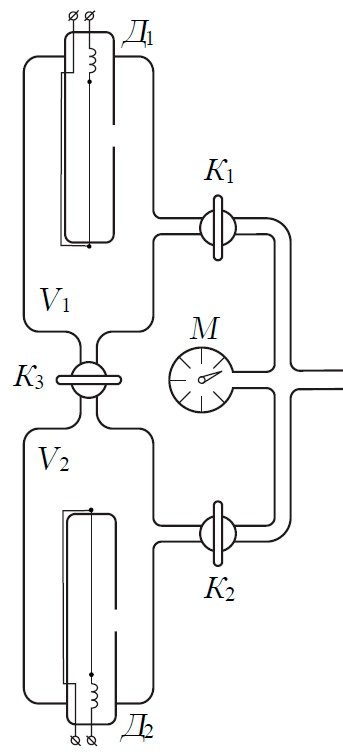
\includegraphics[width=0.9\linewidth]{facility.jpeg}				
		\caption{Схема установки}
	\end{wrapfigure}
	Здесь $V_1,\; V_2$ -- два сосуда с примерно равным объемом, в которые мы будем загонять воздух и гелий.
	
	Данная конструкция позволяет провести диффузию, которая возможна только при равенстве давлений.
	
	Основное оборудование, с помощью которого мы будем снимать измерения -- датчики теплопроводности, через которые пропускают ток. Они подключены к мосту, который позволяет нам устанавливать начальное равновесное состояние.
	
	При изменении концентрации в колбах вольтметр покажет нам разность напряжений на датчиках, что, из-за их конструкции, означает разность концентраций. 
	
	С помощью изменения напряжения мы и будем изучать процесс диффузии, т.к. во время ее протекания концентрации газов начинают устанавливаться, что заметно на графике разницы напряжений от времени.
	
    \bigskip
    \textbf{Методика измерений:} 
    \begin{enumerate}
        \item Сбалансируем измерительный мост при начальном давлении 40 торр. согласно тому, как написано в описании работы.
        \item Приготовим рабочие смеси для проведения измерений. В одном сосуде должен быть чистый воздух, в другом смесь воздуха с гелием. 
        \item Процесс диффузии начинается после открывания крана К3. Запускаем компьютерную программу, которая показывает как меняются показания вольтметра с течением времени. Продолжаем измерять пока показания не упадут на половину.
        \item Повторяем для 4-5 различных значениях рабочего давления.
    \end{enumerate}


    \section{Результаты измерений и обработка данных}
    \subsection*{Коэффициент взаимной диффузии}
    Из теоретических сведений
    \[ U=U_0e^{-t/\tau} \] 
    Если построить графики зависимости в виде, то
    \[ ln(U) = ln(U_0) + (-\dfrac{1}{\tau}) \cdot t \]

    \begin{figure}[h]
        \begin{minipage}[h]{0.49\linewidth}
        \center{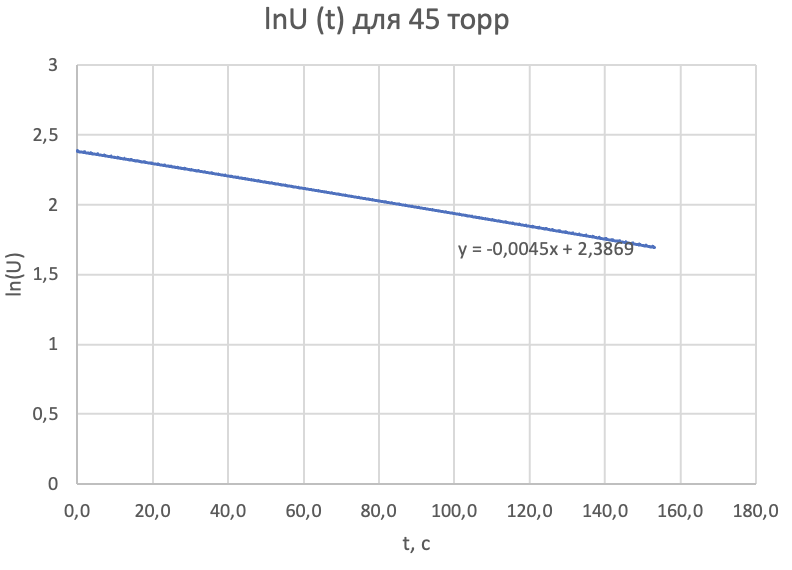
\includegraphics[width=1.08\linewidth]{455.png}}
        \caption{график для 45 торр.}
        \end{minipage}
        \hfill
        \begin{minipage}[h]{0.49\linewidth}
        \center{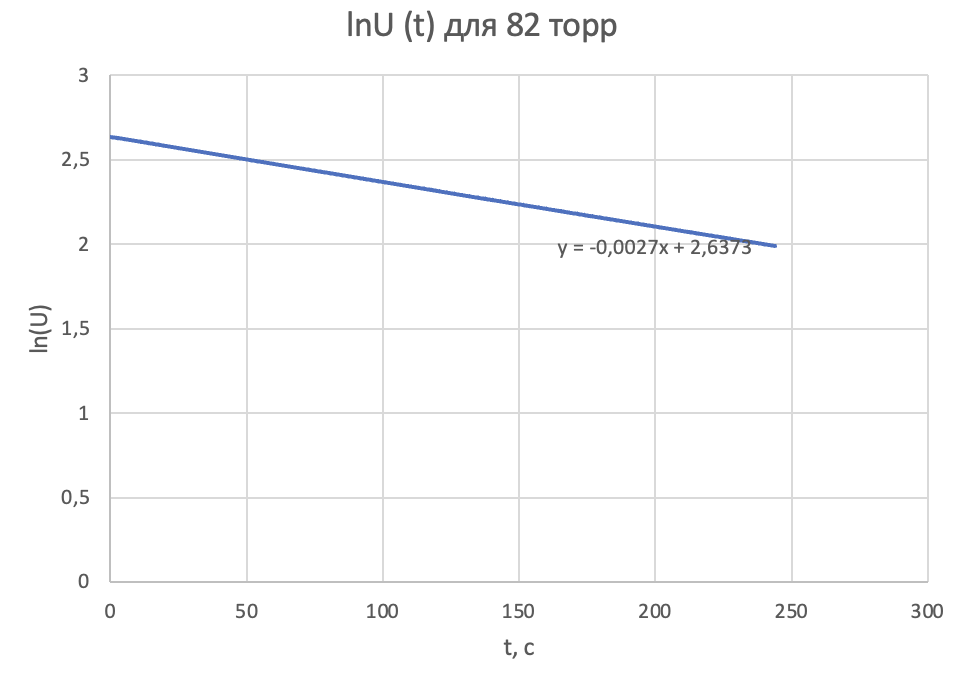
\includegraphics[width=1.1\linewidth]{82.png}}
        \caption{график для 82 торр.}
        \end{minipage}
    \end{figure}

    \begin{figure}[h]
        \begin{minipage}[h]{0.49\linewidth}
        \center{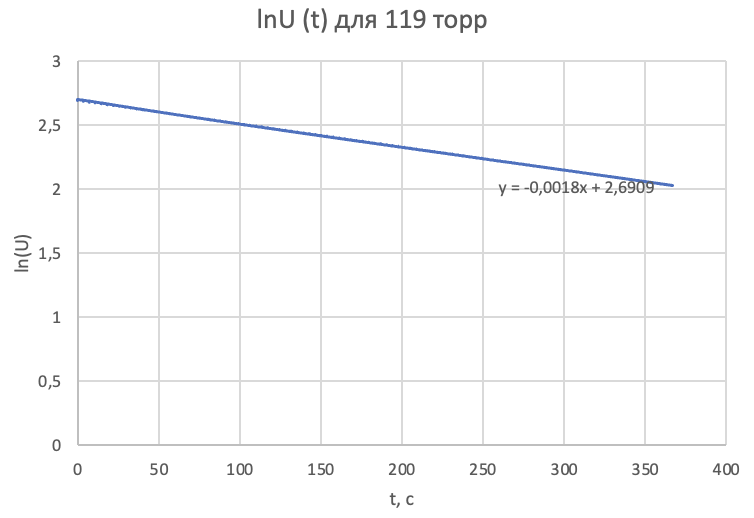
\includegraphics[width=1.1\linewidth]{119.png}}
        \caption{график для 119 торр.}
        \end{minipage}
        \hfill
        \begin{minipage}[h]{0.49\linewidth}
        \center{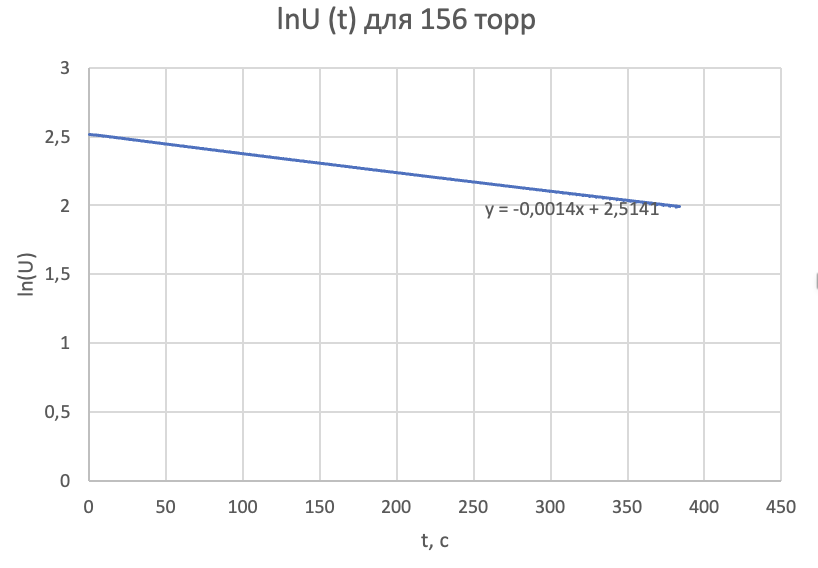
\includegraphics[width=1.12\linewidth]{156.png}}
        \caption{график для 156 торр.}
        \end{minipage}
    \end{figure}

    \begin{figure}[H]
        \centering
        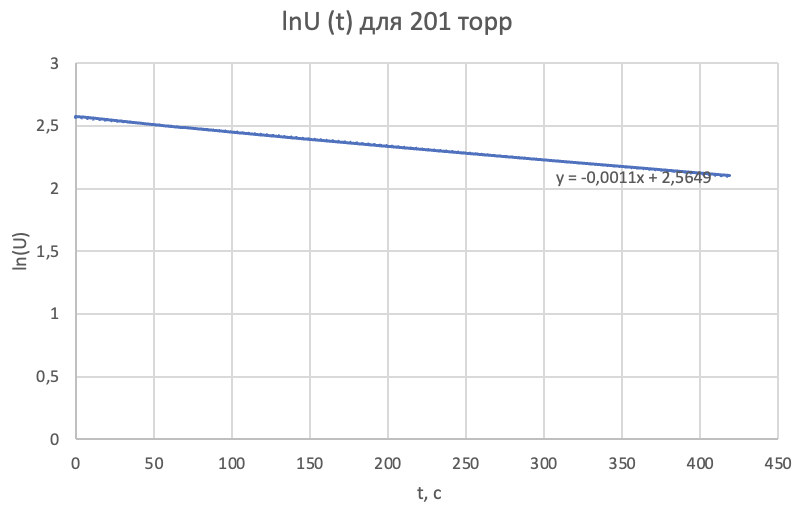
\includegraphics[width=0.6\textwidth]{201.png}
        \caption{график для 201 торр.}
    \end{figure}

    Коэффициент наклона $k$ этих графиков найдем через МНК. Далее $\tau$ выразится как:
    \[ \tau = -\dfrac{1}{k} \]



    Тогда коэффициент взаимной диффузии выразится как
    \begin{align}
		D = \frac{1}{\tau}\frac{VL}{2S} = -k \frac{VL}{2S} & & \sigma_D = D\sqrt{\varepsilon_k^2 + \varepsilon_V^2  + \varepsilon_{\frac{L}{S}}^2}
	\end{align}

    Где параметры установки равны 
    \[ V = (775 \pm 10) \text{ см}^3,\] \[ \frac{L}{S} = (5,3 \pm 0,1) \text{ см}^{-1}. \]
    
    Так как цена деления была равна примерно 3,7 торр, то погрешность измерения давления равна половине цене деления $\sigma_P = 1,9$ торр.
    
    Построим таблицу по полученным данным

    \begin{table}[!h]
        \centering
        \begin{tabular}{|c|c|c|c|c|c|}
            \hline
            $ P $, торр & $ \sigma_P $, торр & $ k $, с$ ^{-1} $ & $ \sigma_{k} \cdot 10^{-6} $, с$ ^{-1} $ & $ D $, $\frac{\text{см}^2}{\text{с}}$ & $ \sigma_D $ $\frac{\text{см}^2}{\text{с}}$ \\ \hline
            45 & 1,9 & -0.0045 & 3 & 9,24 & 0,2 \\ \hline
            82& 1,9 & -0.0027 & 1 & 5.55 & 0,1 \\ \hline
            119 & 1,9 & -0,0018 & 2 & 3,70 & 0,1 \\ \hline
            156 & 1,9 & -0.0014 & 1 & 2,88 & 0,1 \\ \hline
            201 & 1,9 & -0.0011 & 2 & 2,26 & 0,1 \\ \hline
        \end{tabular}
        \caption{Получение коэффициента взаимной диффузии}
    \end{table}

    \subsection*{График зависимости $D(\dfrac{1}{P})$}

    \begin{table}[!h]
        \centering
        \begin{tabular}{|c|c|c|c|}
            \hline
            $ 1/P \cdot 10^{-3} $, торр$ ^{-1} $  & $ \sigma_{1/P} \cdot 10^{-3} $, торр$ ^{-1} $ & $ D $, $ \frac{\text{см}^2}{\text{с}} $ & $ \sigma_D $, $ \frac{\text{см}^2}{\text{с}} $ \\ \hline
            22,2 & 1,0 & 9,24 & 0,2 \\ \hline
            12,2 & 0,3 & 5,55 & 0,1 \\ \hline
            8,4 & 0,1 & 3,70 & 0,1 \\ \hline
            6,4 & 0,1 & 2,88 & 0,1 \\ \hline
            5,0 & 0,1 & 2,26 & 0,1 \\ \hline
        \end{tabular}
        \caption{Итоговые результаты}
    \end{table}


    \begin{figure}[H]
        \centering
        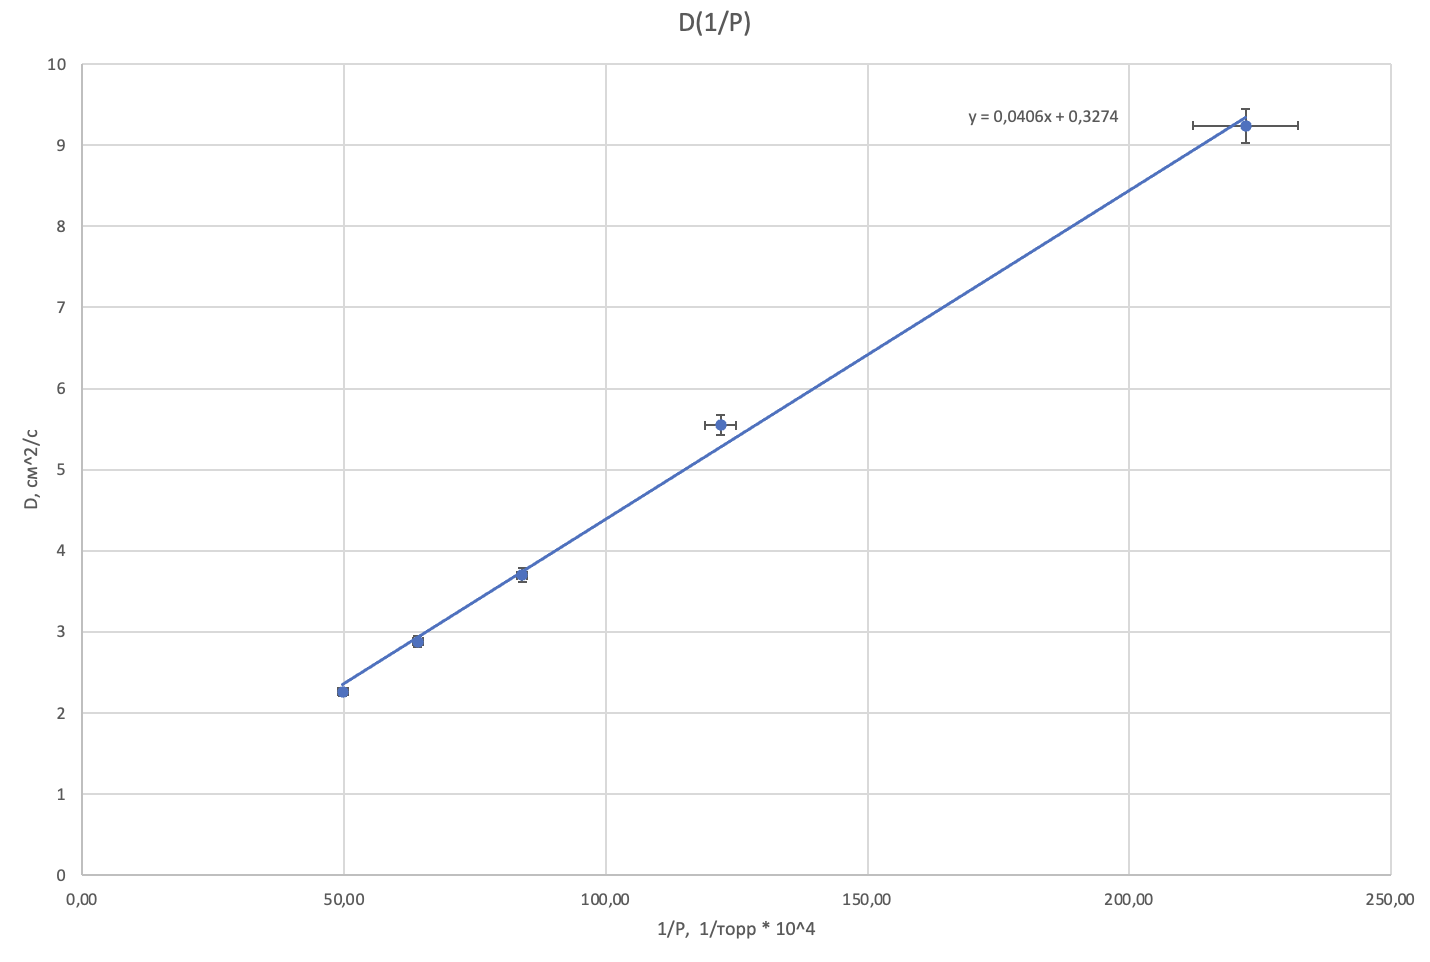
\includegraphics[width=1\textwidth]{graph.png}
        \caption{Зависимость $ D $ от $ \dfrac{1}{P}$}
    \end{figure}

    Построен по МНК, коэффицент наклона $k = (406 \pm 18)\text{ } \frac{\text{см}^2}{\text{с}\cdot\text{торр}}$. 
	
	Значит, коэффициент диффузии при атмосферном давлении $p_{атм} = 754$ торр. можно найти таким образом:\[D_\text{атм} = k\dfrac{1}{P_\text{атм}} = (0,54 \pm0,02)\text{ } \frac{\text{см}^2}{\text{с}}\]
	
	\subsection*{Длина свободного пробега}
	
	По полученным данным оценим длину свободного пробега атомов гелия в воздухе:
	
	\begin{align}
		D=\dfrac{1}{3}\lambda\langle v\rangle,\text{ где } \langle v \rangle = \sqrt{\dfrac{8RT}{\pi \mu}} \Rightarrow \lambda = 3D\sqrt{\dfrac{\pi \mu}{8RT}} = (130\pm 5)\text{ нм}
	\end{align}
	
	\section{Вывод}
	
	В ходе работы:
	
	\begin{enumerate}
		\item Была зарегистрирована зависимость концентрации гелия в воздухе от времени с помощью датчиков теплопроводности при различных начальных давлениях смеси газов. Сначала для 40 торр., потом для 80, 120, 160, 200 торр.
		\item Построив линейный график $lnU (t)$ были найдены коэффициенты взаимной диффузии для 5 различных давлений. Далее нашли коэффициент взаимной диффузии для смеси гелий-воздух при атмосферном давлении: $D_\text{атм} = (0,54\pm0,02)\text{ } \frac{\text{см}^2}{\text{с}}$. Сравним с табличным, который равен $D_\text{табл} = 0,62\text{ } \frac{\text{см}^2}{\text{с}}$. Видно, что табличное значение почти входит в пределы погрешности полученого из лабораторной работы. Небольшое отклонение могло возникнуть в связи не совсем точным измерением давления манометром, т.к например для 40 торр. мы должны были измерять всего 5-6 делений в манометре. Также неточность могла возникнуть из за не совсем хорошей балансировки измерительного моста. Так же наша модель все таки является лишь приближением взаимной диффузии. 
		\item По полученному коэффициенту взаимной диффузии была вычислена длина свободного пробега гелия в воздухе: $\lambda = (130\pm 5)\text{ нм}$. Отклонение могло возникнуть из за причин, описанных выше.
	\end{enumerate}

    \begin{longtable}{|c|c|c|}
        \hline
        $t$, c & ln($U$) & $U$, mV \\
        \hline
        \endhead
        0,0 & 2,38310461 & 10,8385 \\ \hline
        1,0 & 2,378666117 & 10,7905 \\ \hline
        2,1 & 2,374514981 & 10,7458 \\ \hline
        3,1 & 2,37008485 & 10,6983 \\ \hline
        4,1 & 2,365869703 & 10,6533 \\ \hline
        5,1 & 2,361504733 & 10,6069 \\ \hline
        6,1 & 2,357167971 & 10,561 \\ \hline
        7,1 & 2,352755257 & 10,5145 \\ \hline
        8,1 & 2,348494923 & 10,4698 \\ \hline
        9,1 & 2,344062872 & 10,4235 \\ \hline
        10,1 & 2,339745994 & 10,3786 \\ \hline
        11,1 & 2,335313624 & 10,3327 \\ \hline
        12,1 & 2,330803191 & 10,2862 \\ \hline
        13,1 & 2,32651644 & 10,2422 \\ \hline
        14,1 & 2,322005294 & 10,1961 \\ \hline
        15,1 & 2,317513114 & 10,1504 \\ \hline
        16,1 & 2,313149097 & 10,1062 \\ \hline
        17,1 & 2,308587045 & 10,0602 \\ \hline
        18,1 & 2,304363511 & 10,0178 \\ \hline
        19,1 & 2,299791194 & 9,9721 \\ \hline
        20,1 & 2,295429553 & 9,9287 \\ \hline
        21,1 & 2,291018457 & 9,885 \\ \hline
        22,1 & 2,286557332 & 9,841 \\ \hline
        23,1 & 2,282137458 & 9,7976 \\ \hline
        24,1 & 2,277831229 & 9,7555 \\ \hline
        25,1 & 2,273465194 & 9,713 \\ \hline
        26,1 & 2,269038651 & 9,6701 \\ \hline
        27,1 & 2,264509324 & 9,6264 \\ \hline
        28,1 & 2,260105475 & 9,5841 \\ \hline
        29,1 & 2,255703107 & 9,542 \\ \hline
        30,1 & 2,251323377 & 9,5003 \\ \hline
        31,1 & 2,24688209 & 9,4582 \\ \hline
        32,1 & 2,242293541 & 9,4149 \\ \hline
        33,1 & 2,238035905 & 9,3749 \\ \hline
        34,1 & 2,233481501 & 9,3323 \\ \hline
        35,1 & 2,228960081 & 9,2902 \\ \hline
        36,1 & 2,224720844 & 9,2509 \\ \hline
        37,1 & 2,220213843 & 9,2093 \\ \hline
        38,1 & 2,215664621 & 9,1675 \\ \hline
        39,1 & 2,211324702 & 9,1278 \\ \hline
        40,1 & 2,206822811 & 9,0868 \\ \hline
        41,1 & 2,202466371 & 9,0473 \\ \hline
        42,1 & 2,198002053 & 9,007 \\ \hline
        43,1 & 2,193562324 & 8,9671 \\ \hline
        44,1 & 2,189091594 & 8,9271 \\ \hline
        45,1 & 2,184623291 & 8,8873 \\ \hline
        46,1 & 2,180191445 & 8,848 \\ \hline
        47,1 & 2,175512795 & 8,8067 \\ \hline
        48,1 & 2,171211371 & 8,7689 \\ \hline
        49,1 & 2,16674246 & 8,7298 \\ \hline
        50,1 & 2,162184447 & 8,6901 \\ \hline
        51,1 & 2,157848297 & 8,6525 \\ \hline
        52,1 & 2,1532843 & 8,6131 \\ \hline
        53,1 & 2,148839331 & 8,5749 \\ \hline
        54,1 & 2,144280799 & 8,5359 \\ \hline
        55,1 & 2,139772003 & 8,4975 \\ \hline
        56,1 & 2,135337353 & 8,4599 \\ \hline
        57,1 & 2,130871077 & 8,4222 \\ \hline
        58,1 & 2,126527874 & 8,3857 \\ \hline
        59,1 & 2,121974072 & 8,3476 \\ \hline
        60,1 & 2,117567906 & 8,3109 \\ \hline
        61,1 & 2,113093896 & 8,2738 \\ \hline
        62,1 & 2,108587637 & 8,2366 \\ \hline
        63,1 & 2,104158544 & 8,2002 \\ \hline
        64,1 & 2,099685248 & 8,1636 \\ \hline
        65,1 & 2,095253373 & 8,1275 \\ \hline
        66,1 & 2,090739973 & 8,0909 \\ \hline
        67,1 & 2,086305431 & 8,0551 \\ \hline
        68,1 & 2,081701486 & 8,0181 \\ \hline
        69,1 & 2,07716395 & 7,9818 \\ \hline
        70,1 & 2,072832248 & 7,9473 \\ \hline
        71,1 & 2,068380594 & 7,912 \\ \hline
        72,1 & 2,064061371 & 7,8779 \\ \hline
        73,1 & 2,059353624 & 7,8409 \\ \hline
        74,1 & 2,055020767 & 7,807 \\ \hline
        75,1 & 2,050553265 & 7,7722 \\ \hline
        76,1 & 2,04597524 & 7,7367 \\ \hline
        77,1 & 2,041596881 & 7,7029 \\ \hline
        78,1 & 2,037055825 & 7,668 \\ \hline
        79,1 & 2,032520255 & 7,6333 \\ \hline
        80,1 & 2,02799034 & 7,5988 \\ \hline
        81,1 & 2,023347267 & 7,5636 \\ \hline
        82,1 & 2,018895042 & 7,53 \\ \hline
        83,1 & 2,01430284 & 7,4955 \\ \hline
        84,1 & 2,009729662 & 7,4613 \\ \hline
        85,1 & 2,005323954 & 7,4285 \\ \hline
        86,1 & 2,000560659 & 7,3932 \\ \hline
        87,1 & 1,996250132 & 7,3614 \\ \hline
        88,1 & 1,991798147 & 7,3287 \\ \hline
        89,1 & 1,987271427 & 7,2956 \\ \hline
        90,1 & 1,982737891 & 7,2626 \\ \hline
        91,1 & 1,978114547 & 7,2291 \\ \hline
        92,1 & 1,973692061 & 7,1972 \\ \hline
        93,1 & 1,969152233 & 7,1646 \\ \hline
        94,1 & 1,964731903 & 7,133 \\ \hline
        95,1 & 1,96015112 & 7,1004 \\ \hline
        96,1 & 1,95566244 & 7,0686 \\ \hline
        97,1 & 1,951110887 & 7,0365 \\ \hline
        98,1 & 1,94668128 & 7,0054 \\ \hline
        99,1 & 1,942131591 & 6,9736 \\ \hline
        100,1 & 1,93747467 & 6,9412 \\ \hline
        101,1 & 1,933099875 & 6,9109 \\ \hline
        102,1 & 1,928386067 & 6,8784 \\ \hline
        103,1 & 1,9238106 & 6,847 \\ \hline
        104,1 & 1,919243446 & 6,8158 \\ \hline
        105,1 & 1,914611119 & 6,7843 \\ \hline
        106,1 & 1,909957234 & 6,7528 \\ \hline
        107,1 & 1,905400606 & 6,7221 \\ \hline
        108,1 & 1,90101738 & 6,6927 \\ \hline
        109,1 & 1,89641974 & 6,662 \\ \hline
        110,1 & 1,891800863 & 6,6313 \\ \hline
        111,1 & 1,887402927 & 6,6022 \\ \hline
        112,1 & 1,882772551 & 6,5717 \\ \hline
        113,1 & 1,878135922 & 6,5413 \\ \hline
        114,1 & 1,873446977 & 6,5107 \\ \hline
        115,1 & 1,868797668 & 6,4805 \\ \hline
        116,1 & 1,864188652 & 6,4507 \\ \hline
        117,1 & 1,859776309 & 6,4223 \\ \hline
        118,1 & 1,855453884 & 6,3946 \\ \hline
        119,1 & 1,850688537 & 6,3642 \\ \hline
        120,1 & 1,845995097 & 6,3344 \\ \hline
        121,1 & 1,841438127 & 6,3056 \\ \hline
        122,1 & 1,836892159 & 6,277 \\ \hline
        123,1 & 1,832437453 & 6,2491 \\ \hline
        124,1 & 1,827898516 & 6,2208 \\ \hline
        125,1 & 1,823371179 & 6,1927 \\ \hline
        126,1 & 1,818742141 & 6,1641 \\ \hline
        127,1 & 1,814189361 & 6,1361 \\ \hline
        128,1 & 1,809566643 & 6,1078 \\ \hline
        129,1 & 1,805136266 & 6,0808 \\ \hline
        130,1 & 1,800372272 & 6,0519 \\ \hline
        131,1 & 1,79575149 & 6,024 \\ \hline
        132,1 & 1,791309368 & 5,9973 \\ \hline
        133,1 & 1,786663172 & 5,9695 \\ \hline
        134,1 & 1,782113092 & 5,9424 \\ \hline
        135,1 & 1,777457685 & 5,9148 \\ \hline
        136,1 & 1,772967331 & 5,8883 \\ \hline
        137,1 & 1,768405544 & 5,8615 \\ \hline
        138,1 & 1,763600021 & 5,8334 \\ \hline
        139,1 & 1,759132966 & 5,8074 \\ \hline
        140,1 & 1,75455938 & 5,7809 \\ \hline
        141,1 & 1,749930023 & 5,7542 \\ \hline
        142,1 & 1,745418803 & 5,7283 \\ \hline
        143,1 & 1,740887139 & 5,7024 \\ \hline
        144,1 & 1,736422924 & 5,677 \\ \hline
        145,1 & 1,731584746 & 5,6496 \\ \hline
        146,1 & 1,727043155 & 5,624 \\ \hline
        147,1 & 1,722248606 & 5,5971 \\ \hline
        148,1 & 1,717933509 & 5,573 \\ \hline
        149,1 & 1,713076947 & 5,546 \\ \hline
        150,1 & 1,708722004 & 5,5219 \\ \hline
        151,1 & 1,704147912 & 5,4967 \\ \hline
        152,1 & 1,699461415 & 5,471 \\ \hline
        153,1 & 1,694918118 & 5,4462 \\ \hline
        \caption{Таблица измерений для 45 торр.}
    \end{longtable}
        




    
\end{document}